% EDIT HERE
% Enter team number below ??
\newcommand{\TeamNo}{31}
% Enter HW number below ??
\newcommand{\HWno}{01}
% 1st student information
\newcommand{\AuthorOneName}{Merve Nur Öztürk}
\newcommand{\AuthorOneID}{2311322}
% 2nd student information (leave empty if none)
\newcommand{\AuthorTwoName}{Atakan Süslü}
\newcommand{\AuthorTwoID}{2311371}
% 3rd student information (leavIDnumber1e empty if none)
\newcommand{\AuthorThreeName}{Betül Rana Kuran}
\newcommand{\AuthorThreeID}{2311173}
% END EDITING
% DO NOT MODIFY BELOW EXCEPT FOR ADDING PACKAGES #######
\documentclass[letterpaper,12pt]{article}
\usepackage{tabularx} % extra features for tabular environment
\usepackage{amsmath}  % improve math presentation
\usepackage{amssymb}
\usepackage{xcolor}
\usepackage{float}
\usepackage[export]{adjustbox}
\usepackage{graphicx} % takes care of graphic including machinery
\usepackage[margin=1in,letterpaper]{geometry} % decreases margins
\usepackage{cite} % takes care of citations

\begin{document}
\begin{center}
AE 305, 2020-21 Fall \hfill \textbf{HW \HWno} \hfill \textbf{Team \TeamNo} \\
\noindent\rule{\textwidth}{0.4pt}
\begin{tabular}{p{0.33\textwidth} | p{0.33\textwidth} | p{0.33\textwidth} }
	\AuthorOneName&\AuthorTwoName&\AuthorThreeName\\
	\textit{\AuthorOneID}&\textit{\AuthorTwoID}&\textit{\AuthorThreeID}
\end{tabular}
\noindent\rule{\textwidth}{0.4pt}
\end{center}

%Report start

\section{Introduction}

It is useful to use numerical methods in order to solve differential equations when
the analytical solution is time-consuming. In this homework, we are given an aircraft
which rolls on the ground and takes off some time later, and we are asked to find
the minimum time required for this aircraft to take off at different airport altitudes.
We know that the aircraft will take off when the lift force is greater than the weight of
the aircraft. Since the lift force is a function of velocity;

\begin{equation}
        L = C_L \cdot \frac{1}{2} \cdot \rho_{\infty} \cdot V_{\infty}^{2} \cdot S
\end{equation}

where the lift coefficient $C_L$ is assumed to be constant and equal to the maximum lift coefficient
($C_{L,max} = 1.792$), first, we should calculate velocity which is described in a differential form for
this problem using the force balance equation in the horizontal direction:

\begin{equation}
        \frac{W}{g} \cdot \frac{dV}{dt} = T - D - \mu \cdot (W - L)
\end{equation}

where the lift and drag forces are initially zero. The next values of drag force are calculated
by this formula:

\begin{equation}
        D = C_D \cdot \frac{1}{2} \cdot \rho_{\infty} \cdot V_{\infty}^{2} \cdot S
\end{equation}

The drag coefficient $C_D$ is also assumed to be constant ($C_D = 0.215$) and its value is 
calculated by this equation;

\begin{equation}
        C_D = 0.0207 + 0.0605C_L^{2}
\end{equation}
        
Therefore, we are asked to use Euler's and RK2 methods so that we can approach the
solution with the help of numerical methods.


\section{Method}
Euler's method can be defined as the first-order Taylor Series Expansion. In this method, the space between
the initial point of the independent variable and the desired next point is divided into discrete points. The 
difference between respective discrete points is named as step size, $\Delta x$. Then, a first-order ordinary
differential equation at the initial point is calculated and treated as slope.
\begin{equation}
\frac{dy}{dx} \equiv y \prime \equiv f(x,y) \equiv SLOPE
\end{equation}
The slope is multiplied by the stepsize
and added to the initial dependent variable. The result gave the next dependent variable.

\begin{center}
Next Value = Previous Value + Step Size $\times $ Slope
\end{center}
\begin{equation}
y(x + \Delta x ) = y(x) + \Delta x f(x,y)
\end{equation}
\begin{equation}
y_{i+1} = y_i + \Delta x f(x_i , y_i)
\label{eq:eul}
\end{equation}
This equation was repeated until the $x_i$ exceeded the desired independent point.

Second-Order Runge-Kutta method has a similar equation form with Euler's method:
\begin{equation}
y_{i+1} = y_i + \Delta x \phi (x_i , y_i, \Delta x)
\label{eq:rk2}
\end{equation}
However, in second order RK method, $y\prime $ is not used as slope. In stead of $y\prime $, $\phi$ which is 
called the increment function is used. $\phi$ is weighted slope function over the interval.
\begin{eqnarray}
\phi&=&a_1k_1 + a_2k_2\\
\frac{dy}{dx}&=&f(x,y) \nonumber\\
k_1&=&f(x_i,y_i) \nonumber\\
k_2&=&f(x_i+p_i\Delta x, y_i+p_i\Delta x k_1) \nonumber
\end{eqnarray}
where $p_i<1$  and
We chose $p_i = 2/3 $.
\begin{eqnarray}
a_1+a_2 = 1  \nonumber \\
a_2p_1 = \frac{1}{2} \nonumber 
\end{eqnarray}
Therefore, we found $a_1=1/4$ and $a_2=3/4$ as our weights.
\\\\
Trapezoidal integration rule is a basic version of calculating the area under a curve. It is based on
dividing the area under the curve $y(x)$ into small trapezoids. Then, areas of trapezoids which was equal to 
$\frac {1}{2}(V_i+V_{i+1})\Delta t $ is summed up:
\begin{equation}
\int_{0}^{N_p\Delta t} V(t) dt = \sum_{i=0}^{N_p-1} \frac{1}{2}(V_i+V_{i+1}) \Delta t 
\end{equation}

\newpage

\section{Results and Discussion}

\subsection{Calculation of velocity at sea level with Euler's Method }
\begin{figure}[ht]
\centering 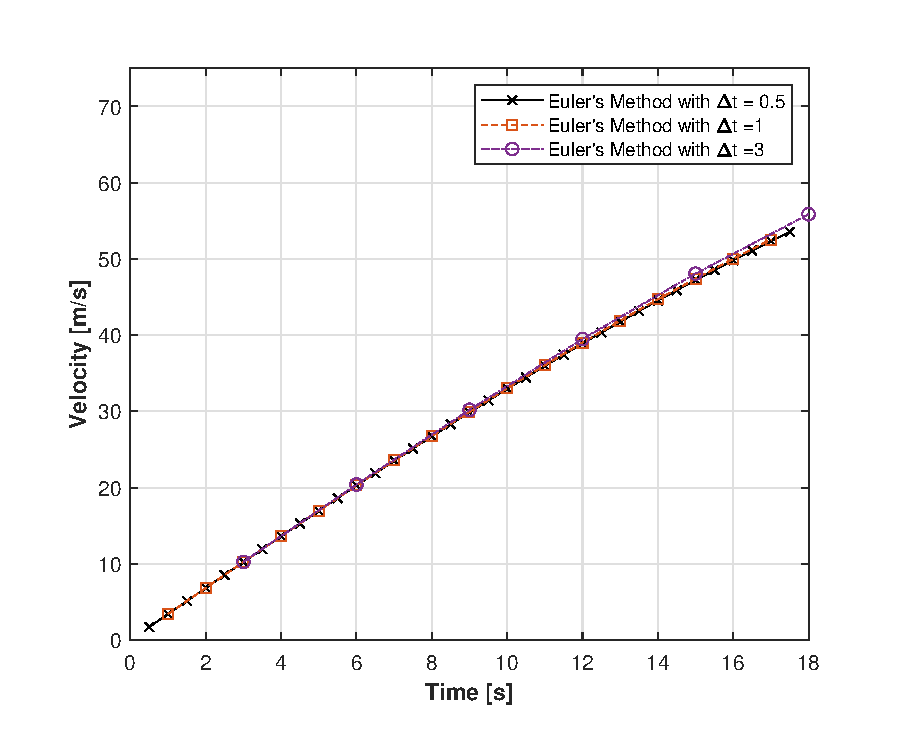
\includegraphics[max height=10cm]{graphs/question1.eps}
\caption{Calculation of velocity using Euler's Method with three different time steps at sea level.}
     \label{fig:q1}
\end{figure}

As can be seen in Figure \ref{fig:q1}, by using different time step sizes, we obtain different results.
Initially, the results were approximately the same for all time step sizes, but as time progresses, the margin of error increases.
This increase occurs at different rates for each time step size. In order to illustrate, when $ \Delta t = 3 $, the
error grows faster than other cases. If we assume that we have the least error when $ \Delta t = 0.5 $, since it is
the smallest time step among all, we can observe that the curves of the other steps deviate more as the time step gets
higher. Thus, when $ \Delta t = 3 $, the result is the least accurate.

\newpage
\begin{figure}[ht]
        \centering 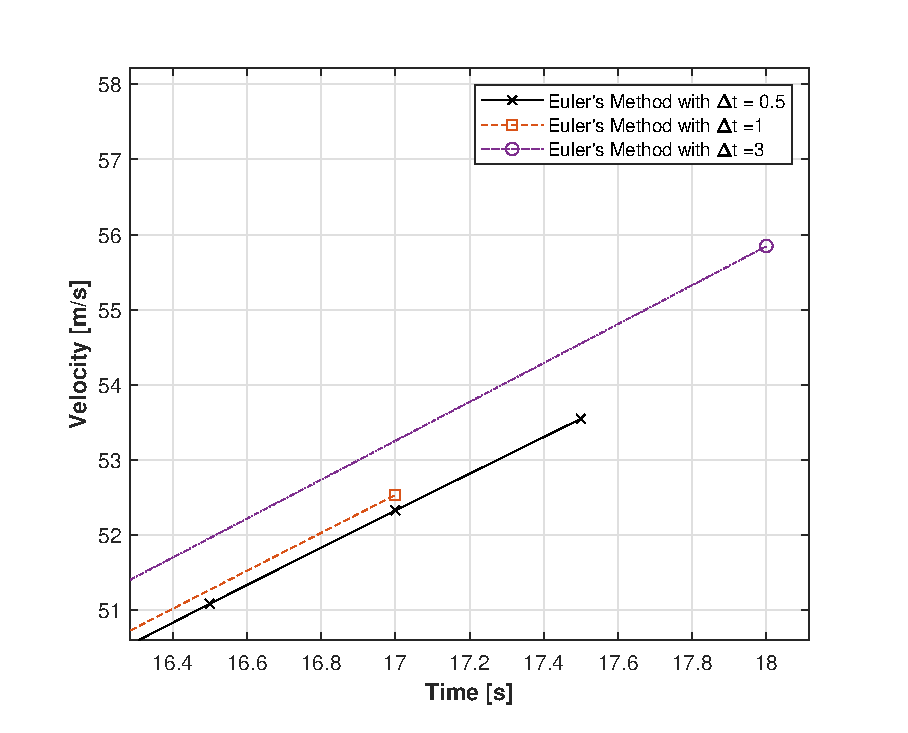
\includegraphics[max height=10cm]{graphs/question1_finaltime.eps}
        \caption{Detailed version of Figure \ref{fig:q1} focused on the endpoints.}
        \label{fig:q1_closer}
\end{figure}

 The effects of using different time step sizes on the result can be clearly seen in Figure \ref{fig:q1_closer}.
 In the first problem of the homework, we were asked to find the minimum time needed for the given aircraft to
 lift off at sea level. When we take a closer look at the curves as we did in Figure \ref{fig:q1_closer}, the
 endpoints, which gives the lift-off time and velocity, are different from each other, and as we mentioned 
 before, we approach the result more precisely for $ \Delta t = 0.5 $. That means if we want to obtain more precise result, 
 we must decrease the step size.
\newpage
\subsection{Calculation of velocity at different altitudes with Euler's Method }
\begin{figure}[ht]
        \centering 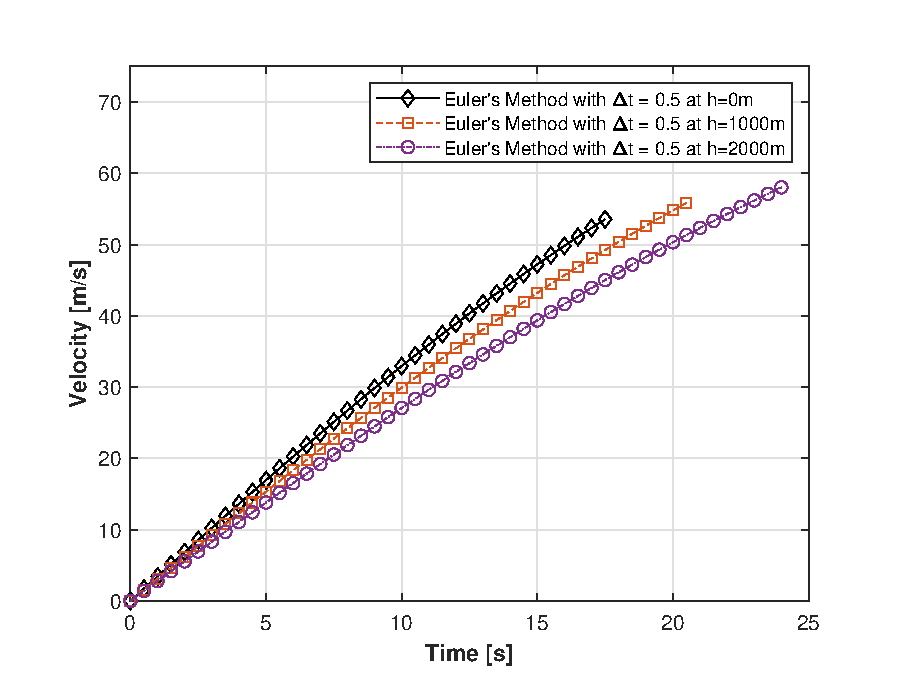
\includegraphics[max height=10cm]{graphs/altitude.eps}
        \caption{Calculated velocities at different altitudes using Euler's method with $\Delta t = 0.5$.}
        \label{fig:altitude}
\end{figure}

It can be obtained from Figure \ref{fig:altitude} that it takes longer for the given aircraft to take off at higher altitudes. 
This is because as the altitude gets higher, the air density decreases, which results in lower maximum available
thrust ($ T_{A,max} = T_{A,max,SL} \frac{\rho_{\infty}}{\rho_{\infty,SL}} $). In addition to that,
lift and drag forces also decrease since they are functions of the free stream air density. The decrease in drag should 
generally result in shorter take-off time while the decrease in thrust and lift force acts exactly the opposite way. However, 
the effect of both the lift force and the thrust overcomes the effect of the drag force. Therefore, take off time increases at higher altitudes.
\newpage
\subsection{Calculation of velocity at sea level with second order RK Method }
\begin{figure}[ht]
        \centering 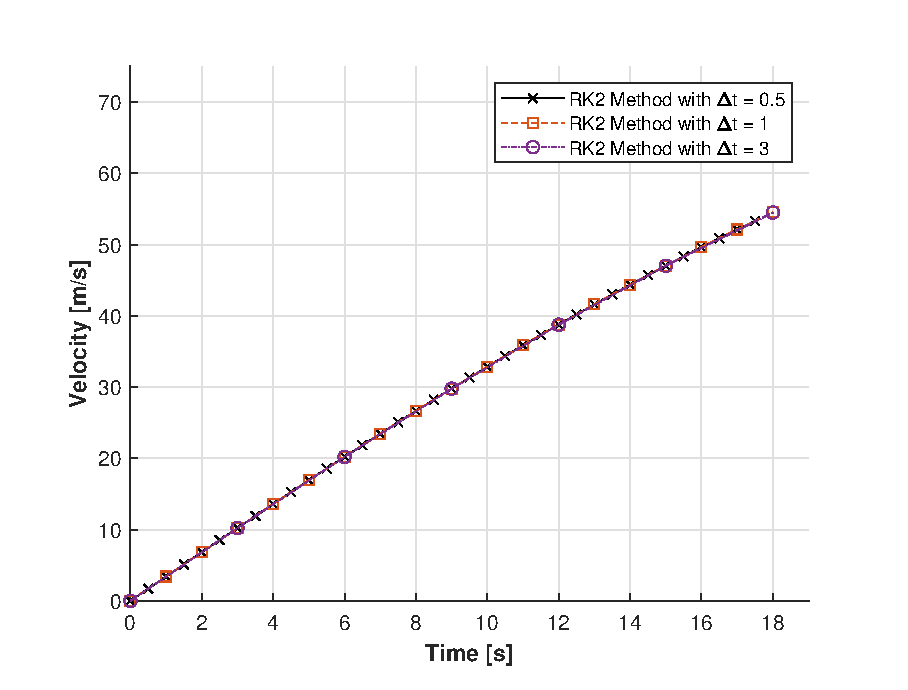
\includegraphics[max height=10cm]{graphs/RK2.eps}
        \caption{Calculated velocities at sea level using second order RK method with different time steps.}
        \label{fig:rk2}
\end{figure}
The results in Figure \ref{fig:rk2} are more similar to each other than Figure \ref{fig:q1}. This is because RK2 method with $p_i=2/3$
is more accurate than Euler's method. In RK2 method with $p_i=2/3$, average slopes at $t_i$ and $t_{i+p_i\Delta t}$
are used instead of using only one slope at $ t_i $ in every iteration. This leads to more stable results than Euler's method 
even with a larger step size. In our case, error became significant only at the endpoints. That error has happened because
algorithm jumps to the next time step even if the true result is closer to the current evaluation point than the next evaluation point.
To decrease this error at the endpoints, a smaller time step must be used.
\newpage
\subsection{Comparison of Euler's method and RK2 method at sea level with different time steps}
\begin{figure}[ht]
        \centering 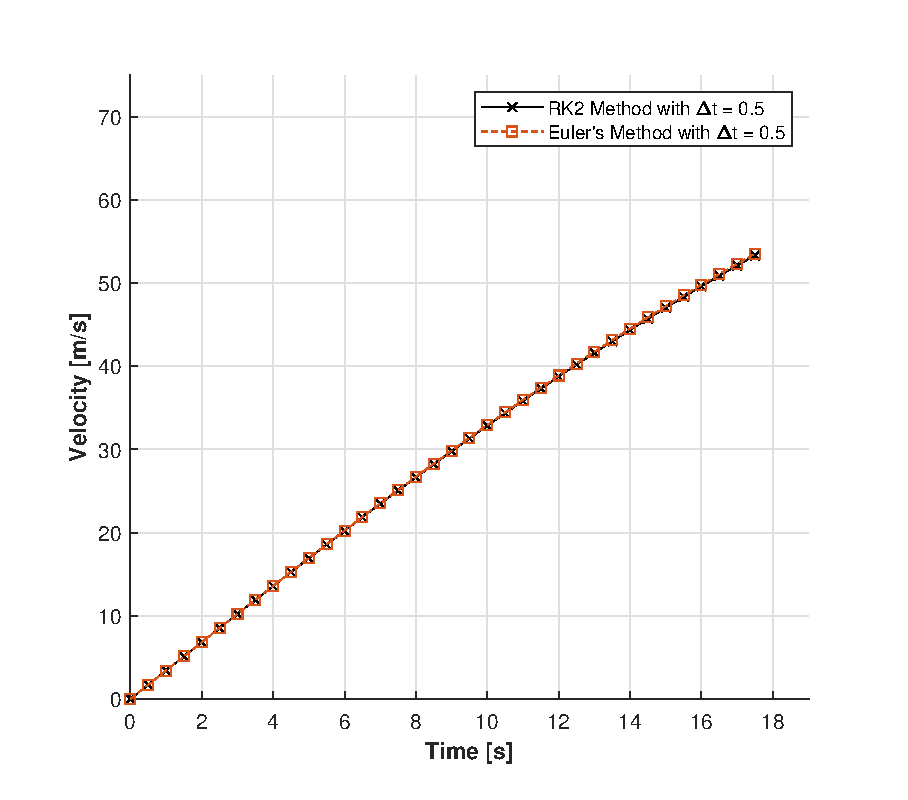
\includegraphics[max height=10cm]{graphs/compare05.eps}
        \caption{Calculated velocities at sea level using second order RK method and Euler's method for $\Delta t=0.5$.}
        \label{fig:rk2_05}
\end{figure}
As can be seen from the Figure \ref{fig:rk2_05}, for $\Delta t = 0.5$, results of RK2 method with $p_i=2/3$ and Euler's method
are approximately the same. This is not surprising since the time step size is so small that the margin of error does not change
significantly for different numerical methods, and we gain accurate results for both methods. However, as the step size increases
the accuracy of the result is more reliable for RK2 method.
\newpage
\begin{figure}[!h]
        \centering
        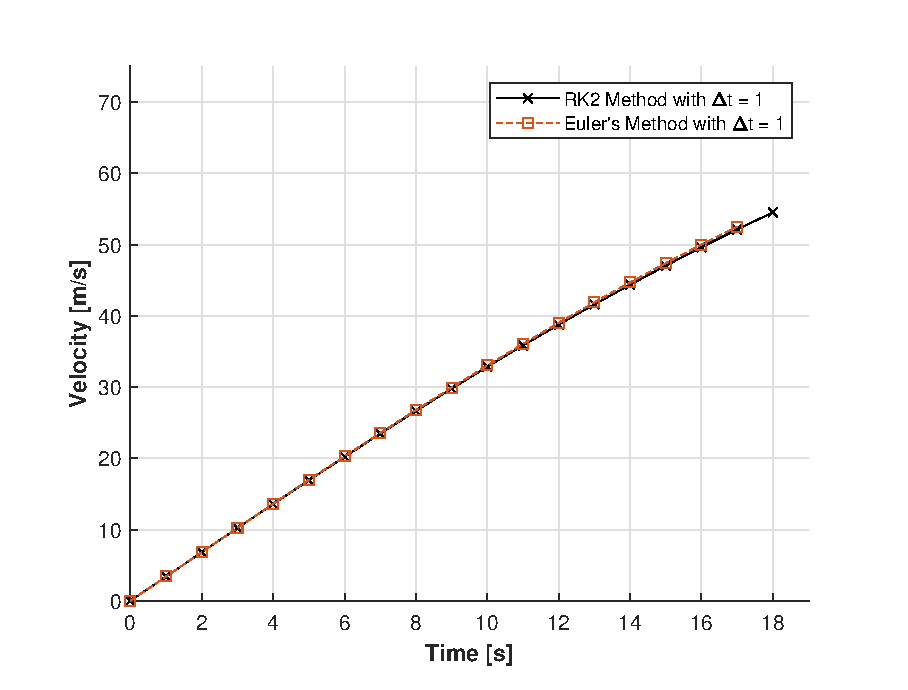
\includegraphics[max height=8cm]{graphs/compare1.eps}
        \caption{Calculated velocities at sea level using second order RK method and Euler's method for $\Delta t=1$.}
        \label{fig:rk2_1}

        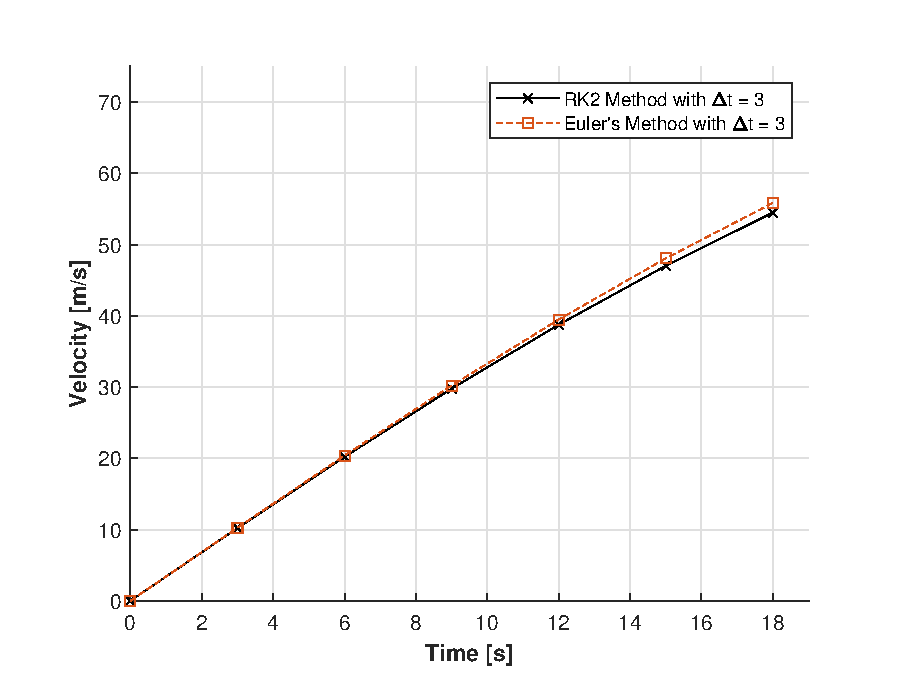
\includegraphics[max height=8cm]{graphs/compare3.eps}
        \caption{Calculated velocities at sea level using second order RK method and Euler's method for $\Delta t=3$.}
        \label{fig:rk2_3}
\end{figure}
The Figures \ref{fig:rk2_1} and \ref{fig:rk2_3} show that increasing step size caused the increase in the 
difference between the results of Euler's method and RK2. This is another proof of larger step sizes leads to an increase in error.
The RK2 method has less truncation error than the Euler's method; therefore, it is more accurate than Euler's method with bigger 
time steps.  

\newpage
\subsection{Calculation of ground roll distance at different altitudes}

\begin{table}[!h]
        \begin{center}
        \caption{Take-off distance $x$ for different altitudes.}
        \vspace{1em}
        \label{tbl:takeoff}
        \begin{tabular}{|c|c|} 
        \hline
        \multicolumn{1}{|c|}{\bf{Altitude (m)}} & \multicolumn{1}{c|}{\bf{\textit{x} (m)}} \\
        \hline
        0 &   493.686 \\ \hline
        1000 &   607.273 \\ \hline
        2000 &   772.654 \\ \hline
        \end{tabular}
        \end{center}
        \end{table}

First, velocities were calculated using RK2 Method with $\Delta t = 0.5$, which is the smallest
timestep used in this problem. Then, integral was taken for each interval using Trapezoidal Integration Method.

As can be seen in Table \ref{tbl:takeoff}, at higher altitudes, take off distance increases dramatically.

\section{Conclusion}
We have calculated minimum take-off time using Euler's Method and second-order RK Method at different altitudes.
We used different time steps for each method and compared the effect of different time step sizes. 

Our computations demonstrated that second-order RK Method gives more reliable results than Euler's Method
when computed with bigger step sizes. We observed that using smaller time step sizes minimizes the effect of truncation error
caused by the usage of different numerical methods. Therefore, if small time step sizes are used, there is no 
significant difference between these two numerical methods.

Also, we have shown that at higher altitudes, both minimum take-off time and ground roll distance are longer.
That is because airplane has to reach a higher velocity to take off.
\end{document}